\section*{Exercício 1}
O banco \texttt{claims} contém 996 apólices de seguro de veículos (de Jong e Heller, 2008). A variável resposta é o custo médio por sinistro, $\texttt{cmsinistros}=\texttt{csinistros}/\texttt{nsinistros}$. As preditoras são \texttt{valorv} e \texttt{expos} (quantitativas) e \texttt{tipov}, \texttt{idadev}, \texttt{sexoc} (no arquivo, \texttt{genero}), \texttt{areac} e \texttt{idadec} (qualitativas). Conforme a OBS1 da lista, não foram ajustados modelos duplos.

\subsection*{Análise descritiva}

\begin{figure}[H]
\centering
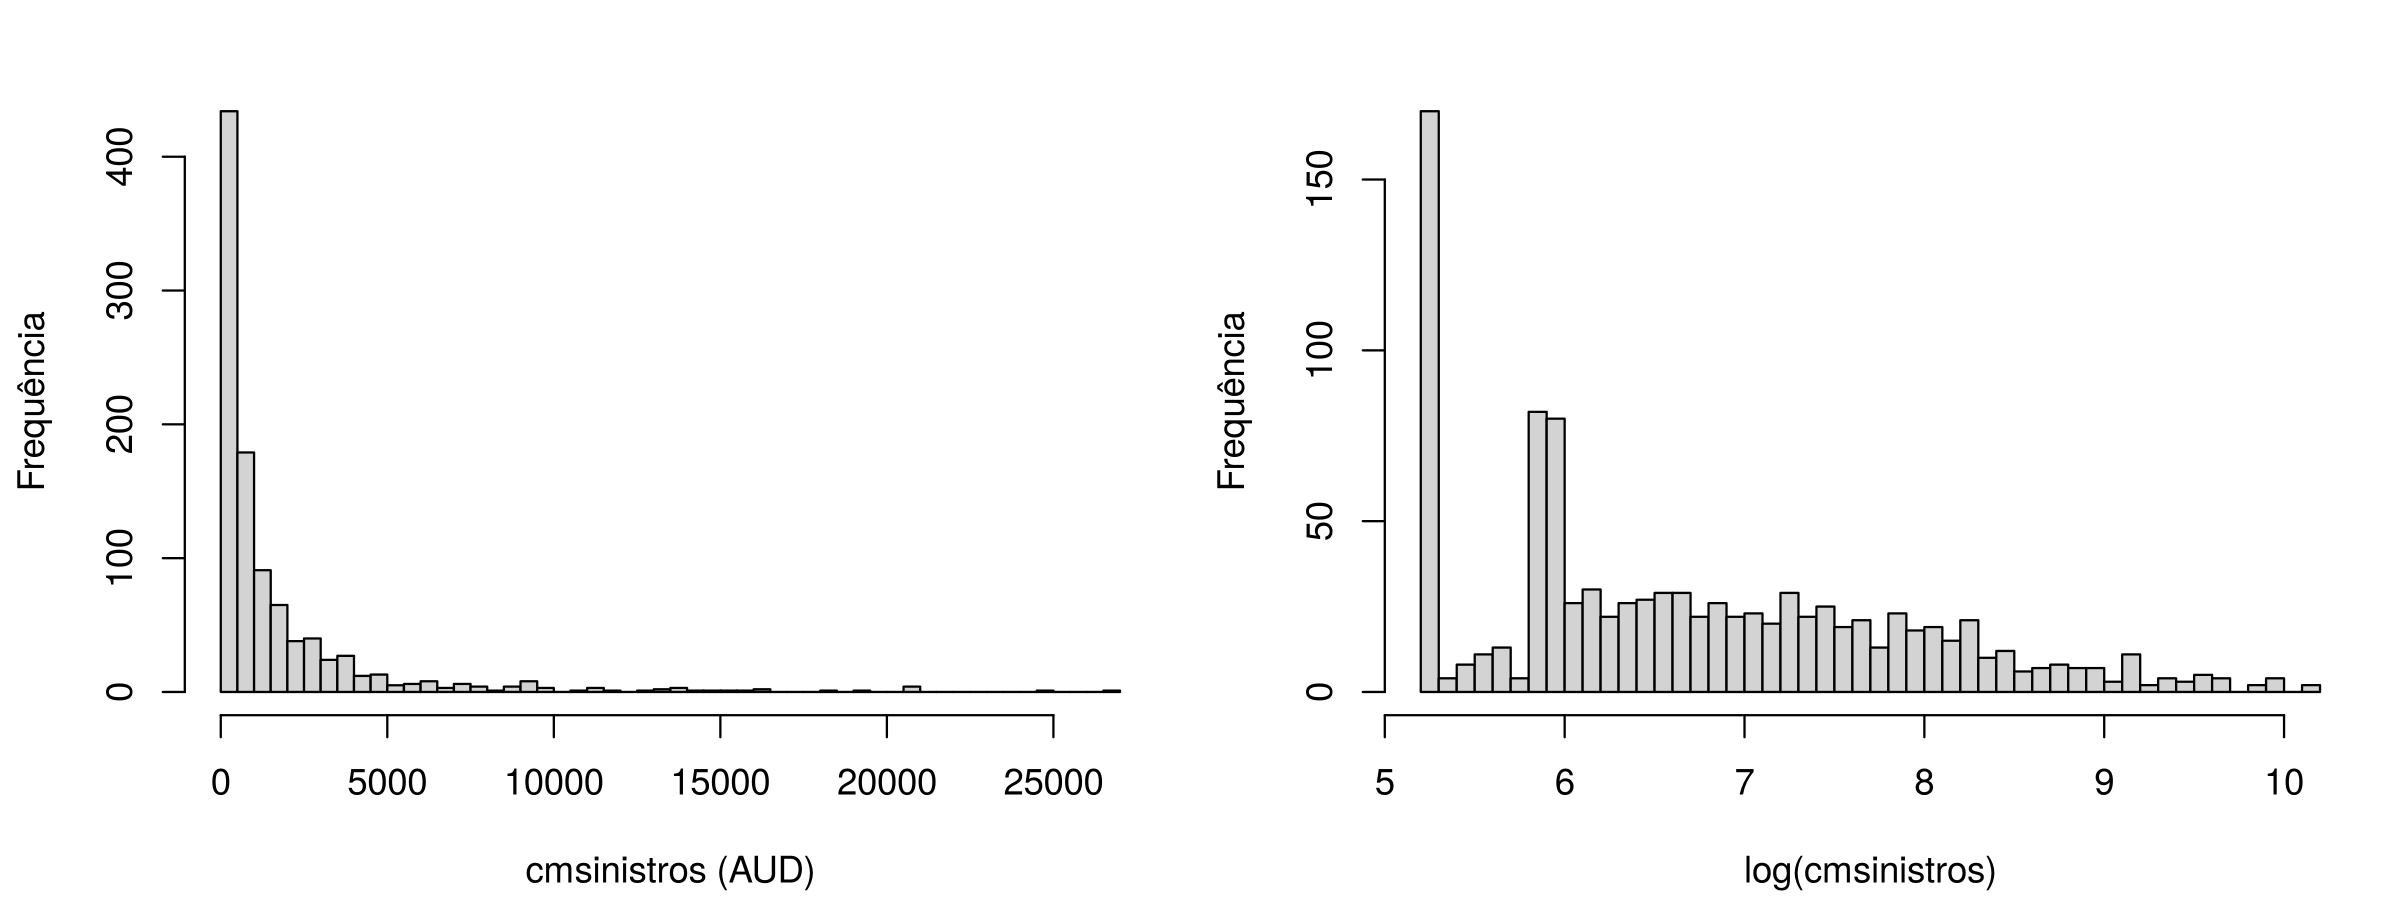
\includegraphics[width=\textwidth]{ex1_resposta.png}
\caption{Histograma de \texttt{cmsinistros} (esquerda) e de $\log(\texttt{cmsinistros})$ (direita).}\label{fig:ex1resp}
\end{figure}

A resposta tem forte assimetria à direita: a média é 1731,3, a mediana é 643,6, o máximo é 26507,3 e o coeficiente de variação é 1,71 (Figura~\ref{fig:ex1resp}). Na escala logarítmica a distribuição fica bem mais simétrica. Isso indica o uso de distribuições para resposta positiva e assimétrica (gama e normal inversa) com ligação logarítmica. Há um detalhe importante nos dados: 163 apólices (16,4\%) têm custo médio igual a 200, exatamente. Esse valor é um piso do banco, e há também acúmulos em torno de 354 e de 390. Além disso, 941 apólices (94,5\%) têm um único sinistro.

\begin{figure}[H]
\centering
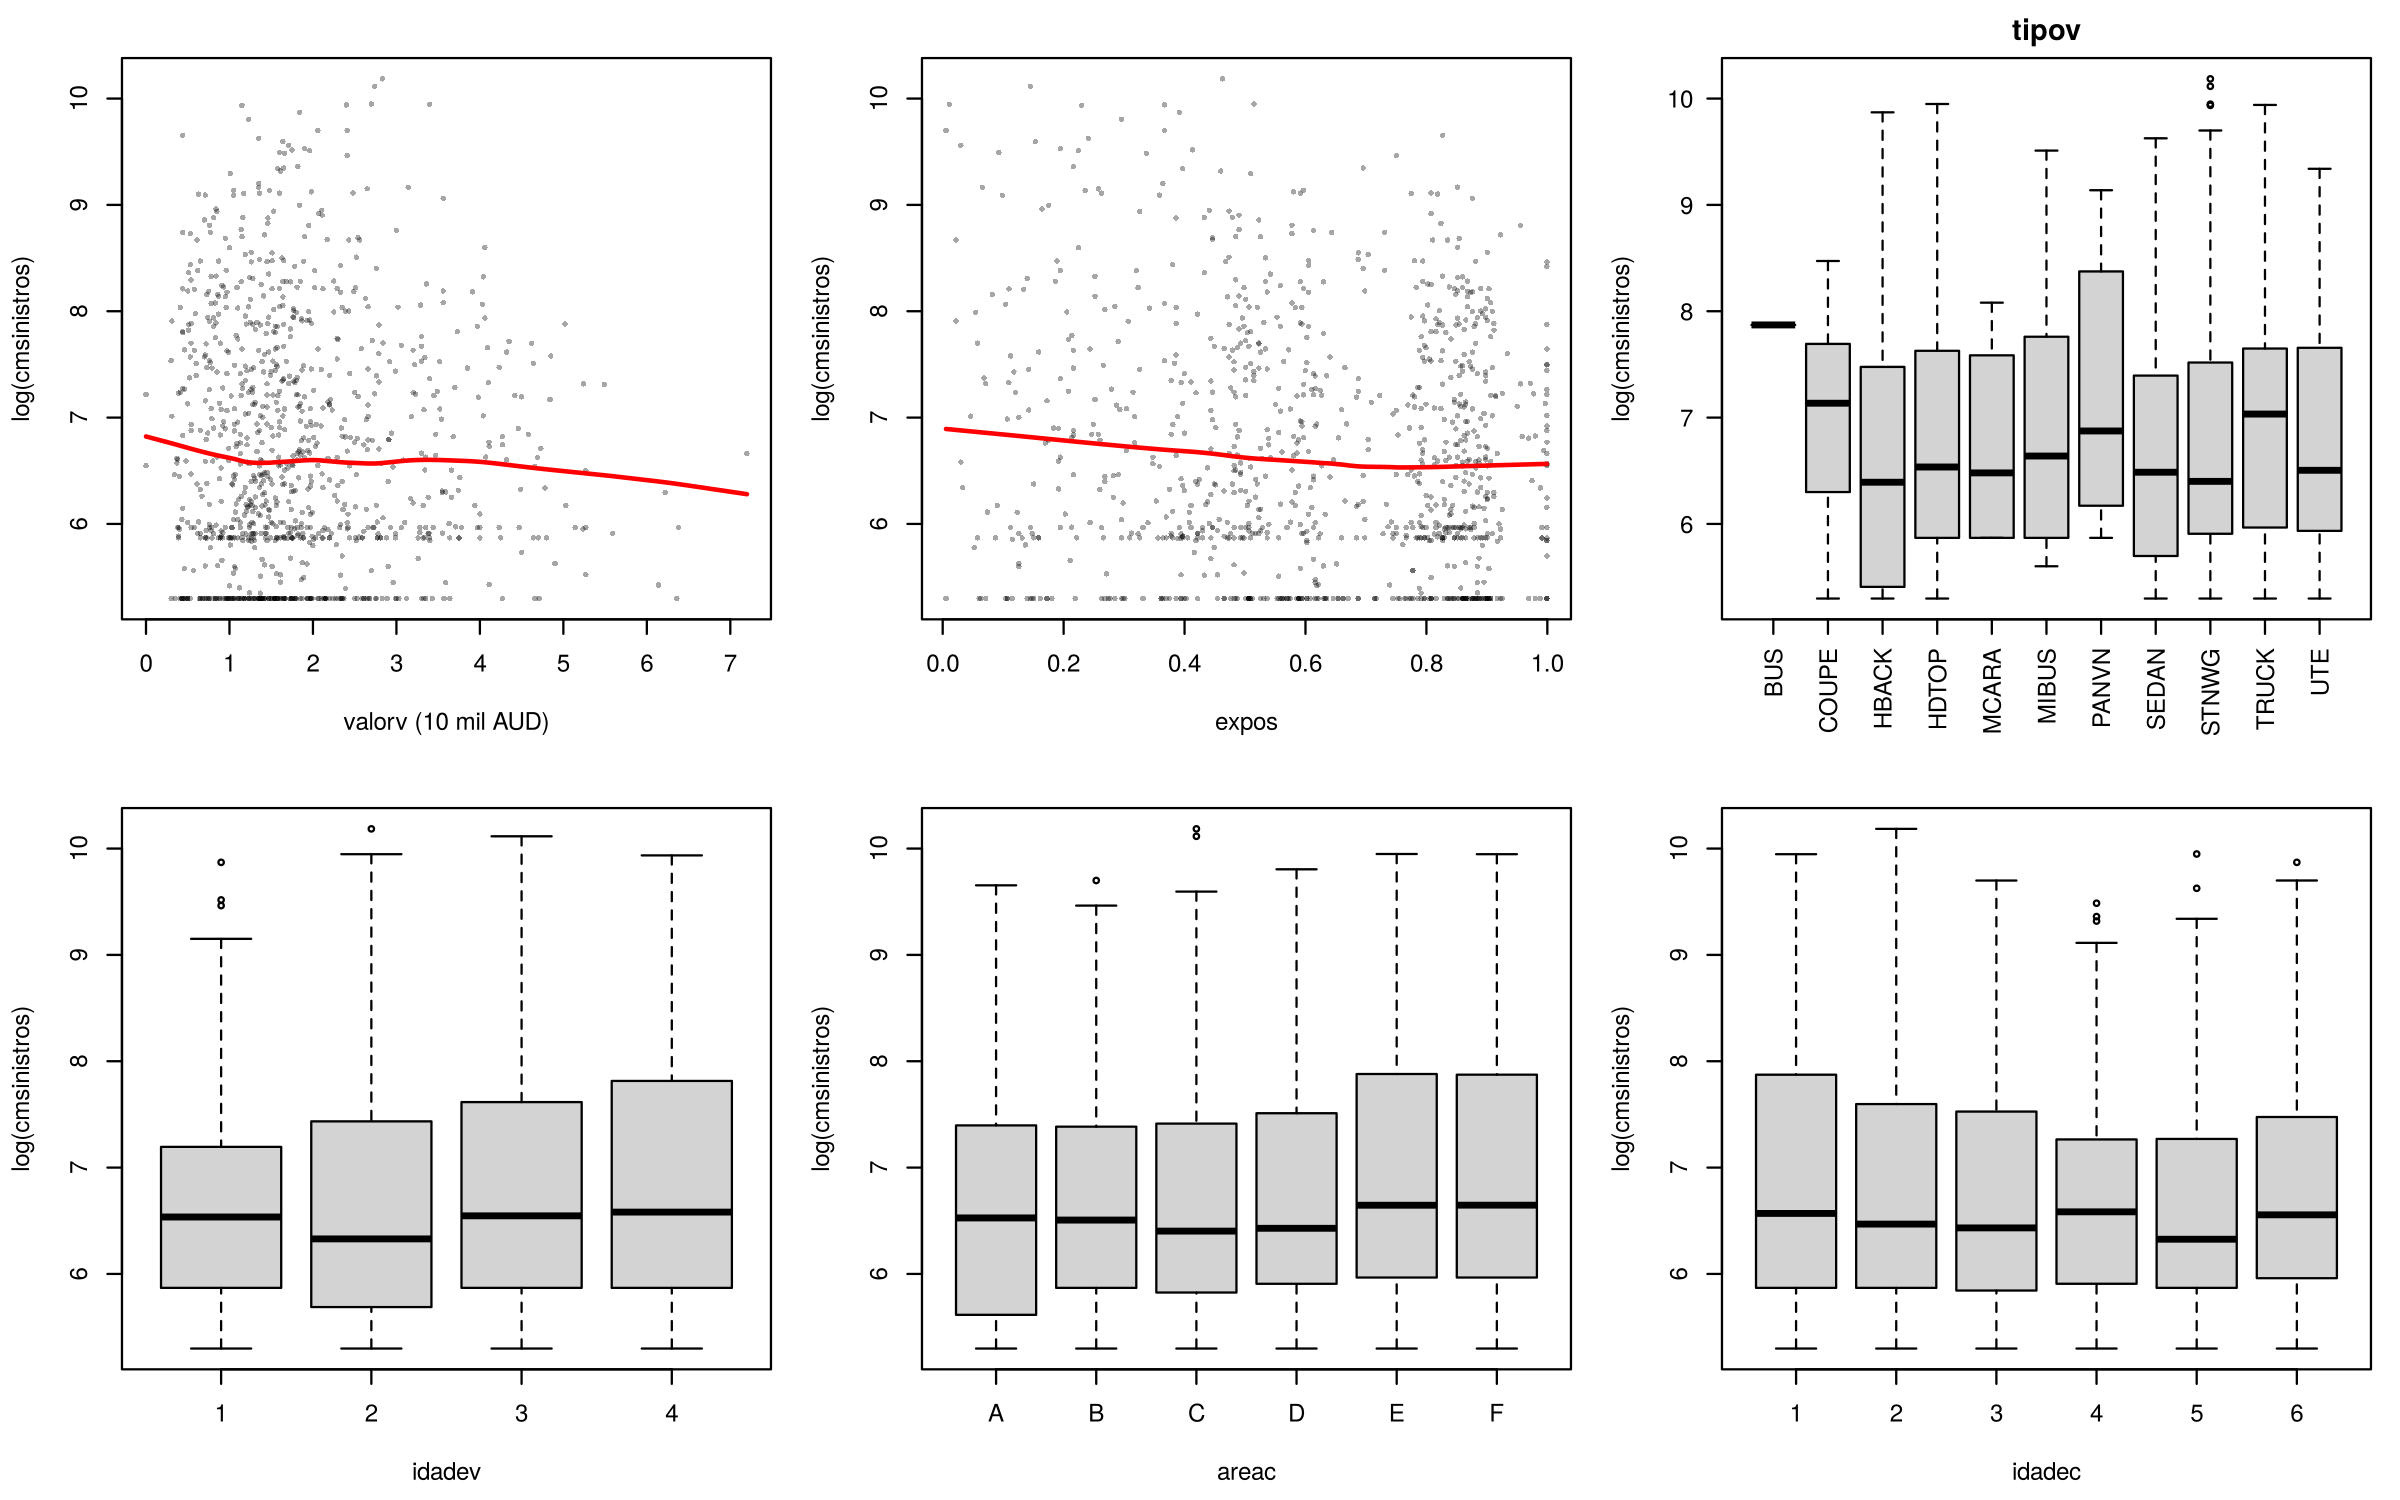
\includegraphics[width=\textwidth]{ex1_preditoras.png}
\caption{$\log(\texttt{cmsinistros})$ contra as preditoras quantitativas (com curva \emph{lowess} em vermelho) e boxplots segundo as preditoras qualitativas.}\label{fig:ex1pred}
\end{figure}

Na Figura~\ref{fig:ex1pred}, \texttt{valorv} não mostra relação clara com o logaritmo do custo, e \texttt{expos} mostra uma leve tendência decrescente. Entre as qualitativas, \texttt{tipov} tem 11 categorias, várias com pouquíssimas observações (BUS com 1, MCARA com 4, MIBUS com 6). As categorias HBACK, SEDAN, STNWG, HDTOP e MCARA têm média do log entre 6,64 e 6,74, enquanto COUPE, MIBUS, PANVN, TRUCK, UTE e BUS ficam acima (6,82 a 7,87). Em \texttt{idadev}, as classes 1 e 2 são parecidas entre si, e as classes 3 e 4 também. Em \texttt{areac}, as áreas A a D são semelhantes (6,62 a 6,72) e as áreas E e F são maiores ($\approx 6{,}95$). Em \texttt{idadec}, o custo tem forma de U: é maior para os condutores mais jovens (1--2) e mais velhos (6) do que para os de idade intermediária (3--5). A diferença entre os sexos é pequena.

\subsection*{Agrupamento das categorias}

Com base nas médias acima, as categorias foram agrupadas como na Tabela~\ref{tab:ex1grp}. Em cada variável, a referência é o grupo com mais observações.

\begin{table}[H]
\centering\small
\caption{Agrupamento das variáveis qualitativas (média de \texttt{cmsinistros} e do seu logaritmo em cada grupo).}\label{tab:ex1grp}
\begin{tabular}{llrrr}
\toprule
Variável & Grupo (categorias originais) & $n$ & Média & Média do log \\
\midrule
\texttt{tipov2} & comum (HBACK, SEDAN, STNWG, HDTOP, MCARA) & 881 & 1662 & 6,663 \\
 & outros (COUPE, MIBUS, PANVN, TRUCK, UTE, BUS) & 115 & 2262 & 6,959 \\
\texttt{idadev2} & 1--2 & 451 & 1591 & 6,611 \\
 & 3--4 & 545 & 1848 & 6,768 \\
\texttt{areac2} & A--D & 850 & 1625 & 6,654 \\
 & E--F & 146 & 2353 & 6,949 \\
\texttt{idadec2} & 3--5 & 592 & 1452 & 6,631 \\
 & 1--2 & 317 & 2119 & 6,776 \\
 & 6 & 87 & 2218 & 6,857 \\
\bottomrule
\end{tabular}
\end{table}

Para verificar se o agrupamento é aceitável, o modelo gama (ligação log) com as categorias originais (27 parâmetros) foi comparado com o modelo com as categorias agrupadas (9 parâmetros) por um teste $F$, já que $\phi$ é estimado. A estatística foi $F=0{,}36$ com 18 e 969 graus de liberdade ($p=0{,}994$). Portanto, o agrupamento não piora o ajuste e as variáveis agrupadas foram usadas daqui em diante.

\subsection*{Seleção de variáveis}

Foi utilizado o método \emph{backward} com teste $F$: parte-se do modelo gama com todas as preditoras (já agrupadas) e, a cada passo, retira-se a variável de maior $p$-valor, desde que ele seja maior que 0,05. Em seguida o modelo é reajustado, porque os $p$-valores das demais variáveis mudam a cada retirada.

\begin{table}[H]
\centering\small
\caption{$p$-valores do teste $F$ para a retirada de cada variável em cada passo do \emph{backward} (modelo gama, ligação log).}\label{tab:ex1step}
\begin{tabular}{lrrr}
\toprule
Variável & Passo 1 & Passo 2 & Passo 3 (final) \\
\midrule
\texttt{genero} & 0,340 & -- & -- \\
\texttt{valorv} & 0,194 & 0,255 & -- \\
\texttt{idadev2} & 0,176 & 0,149 & 0,020 \\
\texttt{tipov2} & 0,009 & 0,005 & 0,007 \\
\texttt{areac2} & $<0{,}001$ & $<0{,}001$ & 0,001 \\
\texttt{idadec2} & $<0{,}001$ & $<0{,}001$ & $<0{,}001$ \\
\texttt{expos} & $<0{,}001$ & $<0{,}001$ & $<0{,}001$ \\
\bottomrule
\end{tabular}
\end{table}

No primeiro passo sai \texttt{genero} ($p=0{,}340$) e no segundo sai \texttt{valorv} ($p=0{,}255$). Com \texttt{valorv} fora do modelo, \texttt{idadev2} passa a ser significativa ($p=0{,}020$), e todas as variáveis restantes ficam significativas (Tabela~\ref{tab:ex1step}). Comparado ao modelo com todas as variáveis agrupadas, o modelo final não perde ajuste ($F=0{,}71$; $p=0{,}493$). O preditor final é
\[
\eta = \beta_0 + \beta_1\,\texttt{expos} + \beta_2\,\texttt{tipov2}_{\text{outros}} + \beta_3\,\texttt{idadev2}_{3\text{--}4} + \beta_4\,\texttt{areac2}_{\text{E--F}} + \beta_5\,\texttt{idadec2}_{1\text{--}2} + \beta_6\,\texttt{idadec2}_{6}.
\]

\subsection*{Diagnóstico do modelo gama}

\begin{figure}[H]
\centering
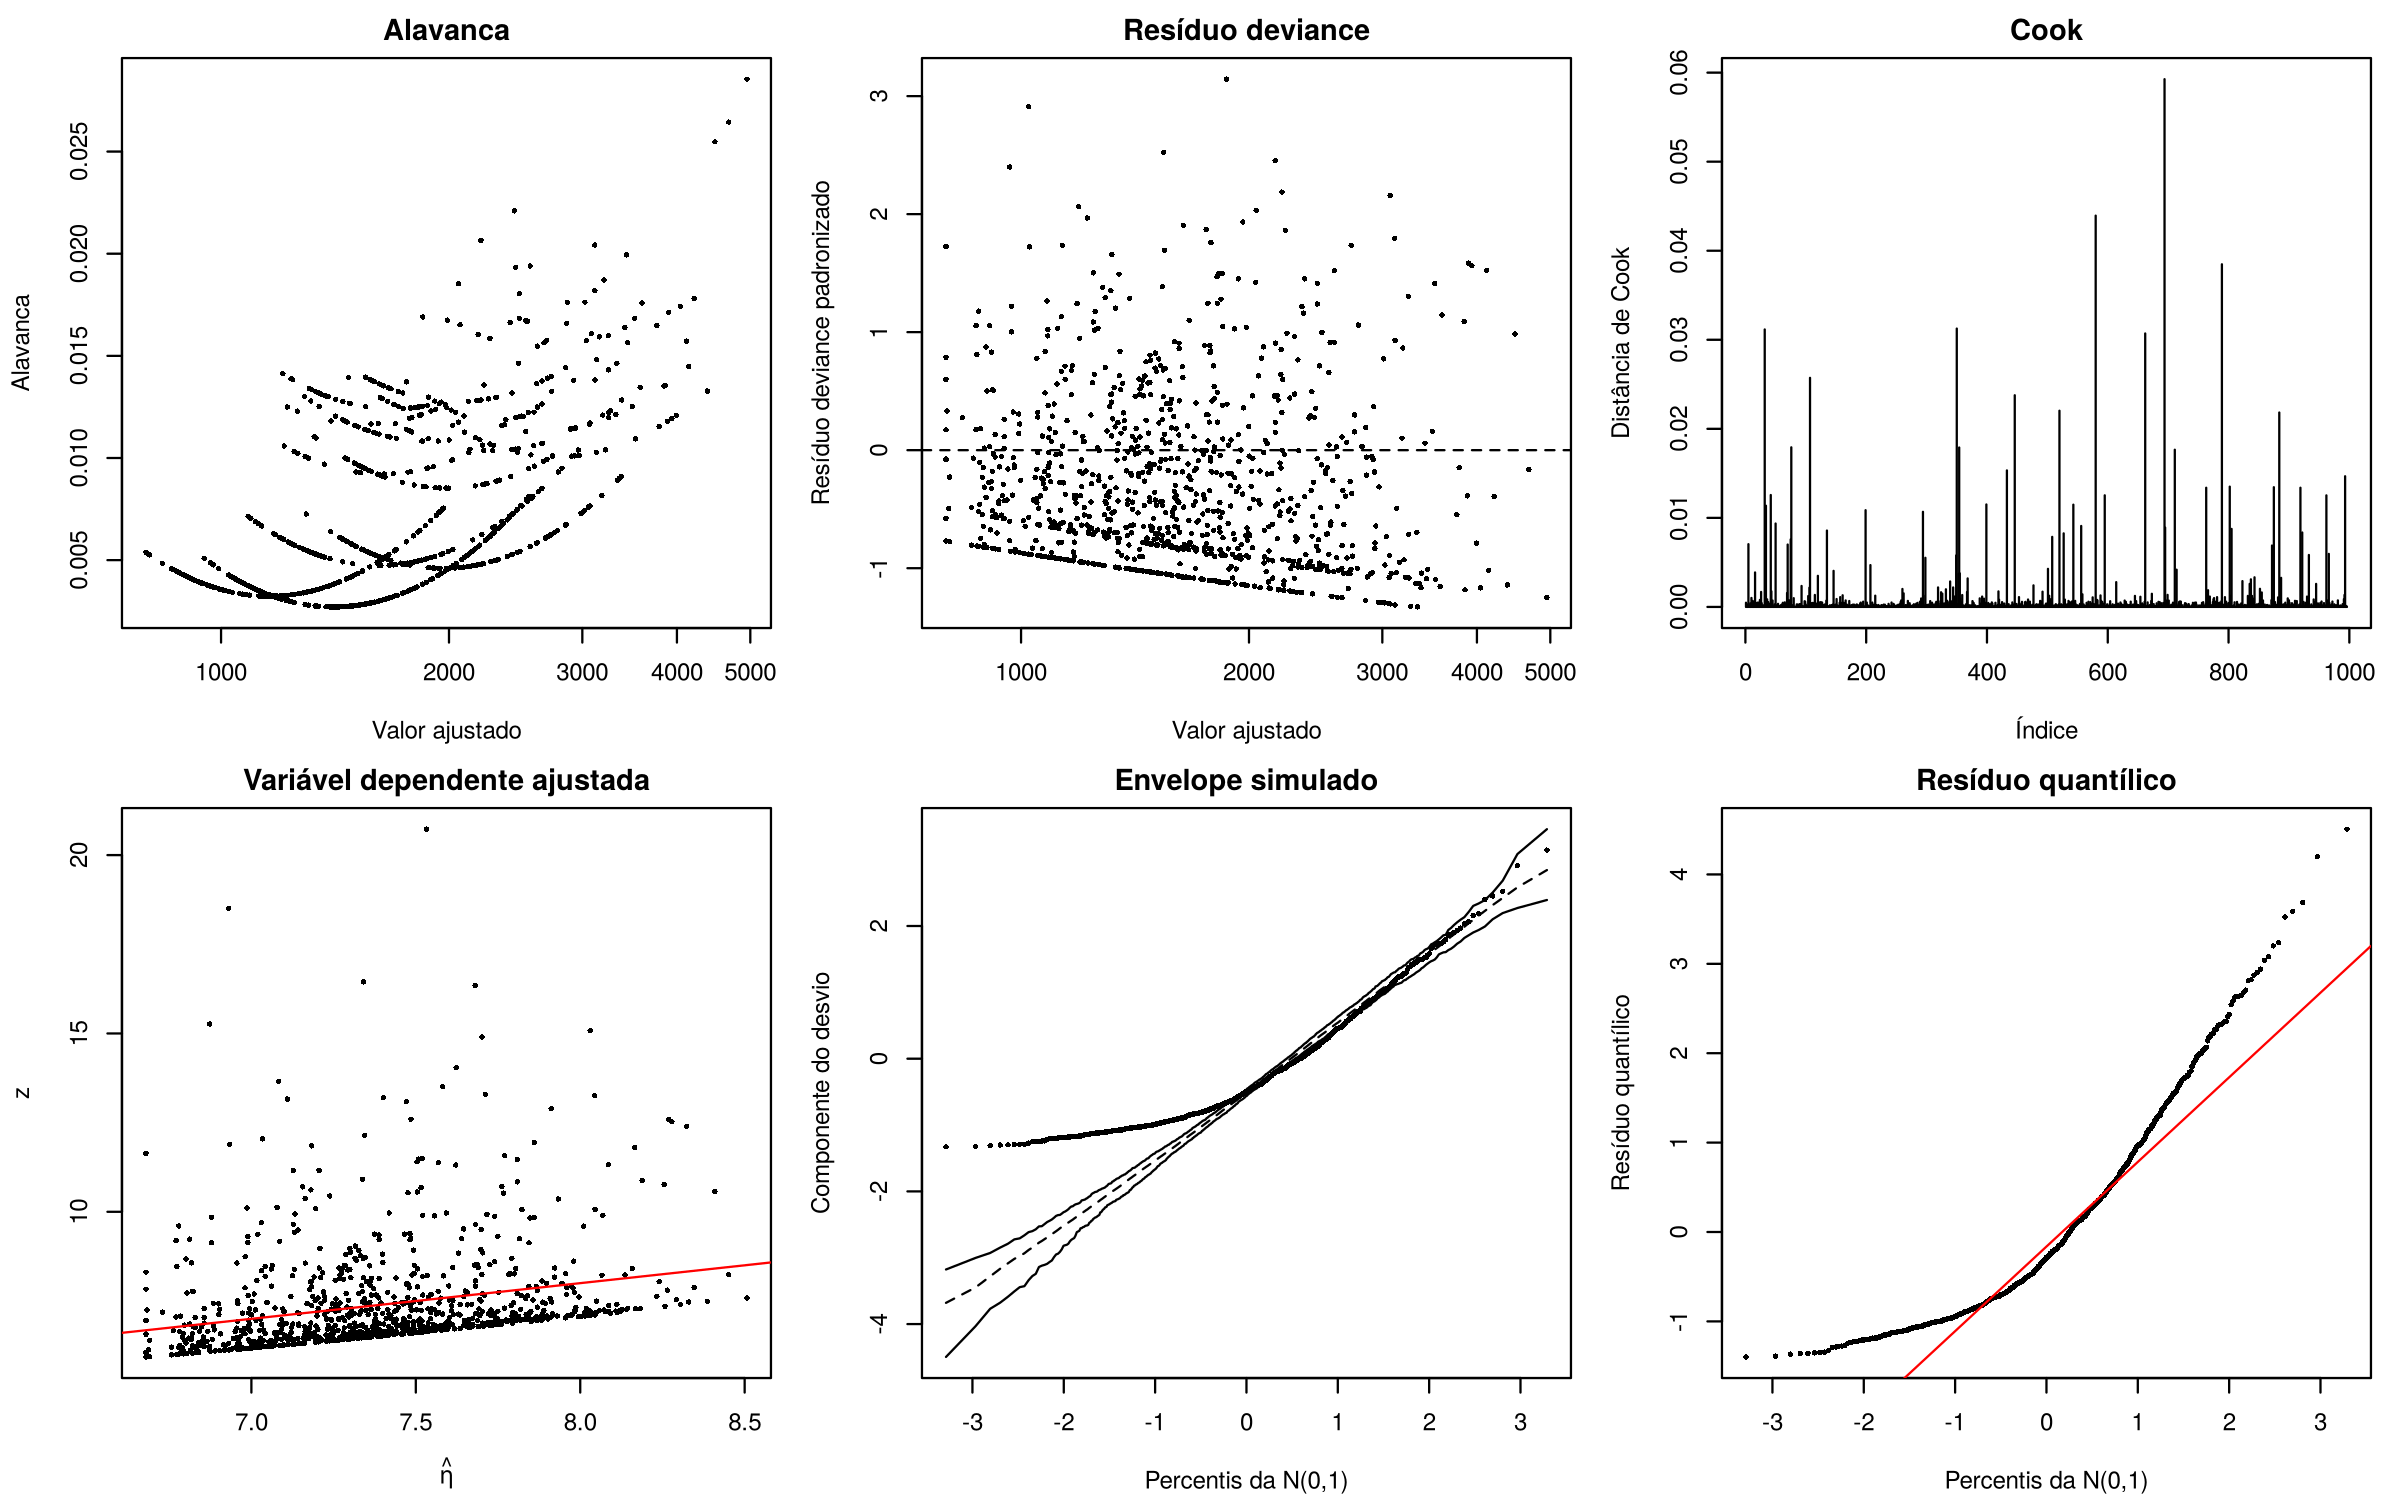
\includegraphics[width=0.92\textwidth]{ex1_diag_gama.png}
\caption{Diagnóstico do modelo gama (ligação log): alavanca, resíduo deviance padronizado, distância de Cook, variável dependente ajustada contra $\hat\eta$, envelope simulado e gráfico normal do resíduo quantílico.}\label{fig:ex1diaggama}
\end{figure}

As alavancas e as distâncias de Cook são pequenas (máximos de 0,029 e 0,059), e nenhum ponto domina o ajuste. O problema está na distribuição. No envelope (Figura~\ref{fig:ex1diaggama}), 64,6\% dos resíduos ficam fora das bandas, e o resíduo quantílico tem assimetria de 1,18, com o gráfico normal bastante curvado. Ou seja, a cauda direita dos dados é mais pesada do que a gama acomoda. As faixas diagonais na parte de baixo do gráfico de resíduos contra valores ajustados correspondem às apólices com custo 200 (e $\approx 354$): para $y$ fixo, o resíduo passa a ser uma função de $\hat\mu$. Conclui-se que o modelo gama não é adequado.

\subsection*{Modelo normal inversa}

O modelo normal inversa com ligação logarítmica foi ajustado com o mesmo preditor. Os coeficientes do modelo gama foram usados como valores iniciais, porque sem eles o algoritmo não converge.

\begin{table}[H]
\centering\small
\caption{Comparação entre os modelos gama e normal inversa (ligação log, mesmo preditor com 7 coeficientes).}\label{tab:ex1comp}
\begin{tabular}{lrrrr}
\toprule
Modelo & AIC & \% fora do envelope & Assimetria do res. quantílico & $p$ de \texttt{idadev2} \\
\midrule
Gama & 16717,5 & 64,6 & 1,18 & 0,020 \\
Normal inversa & 16280,0 & 43,2 & 0,42 & 0,057 \\
\bottomrule
\end{tabular}
\end{table}

\begin{figure}[H]
\centering
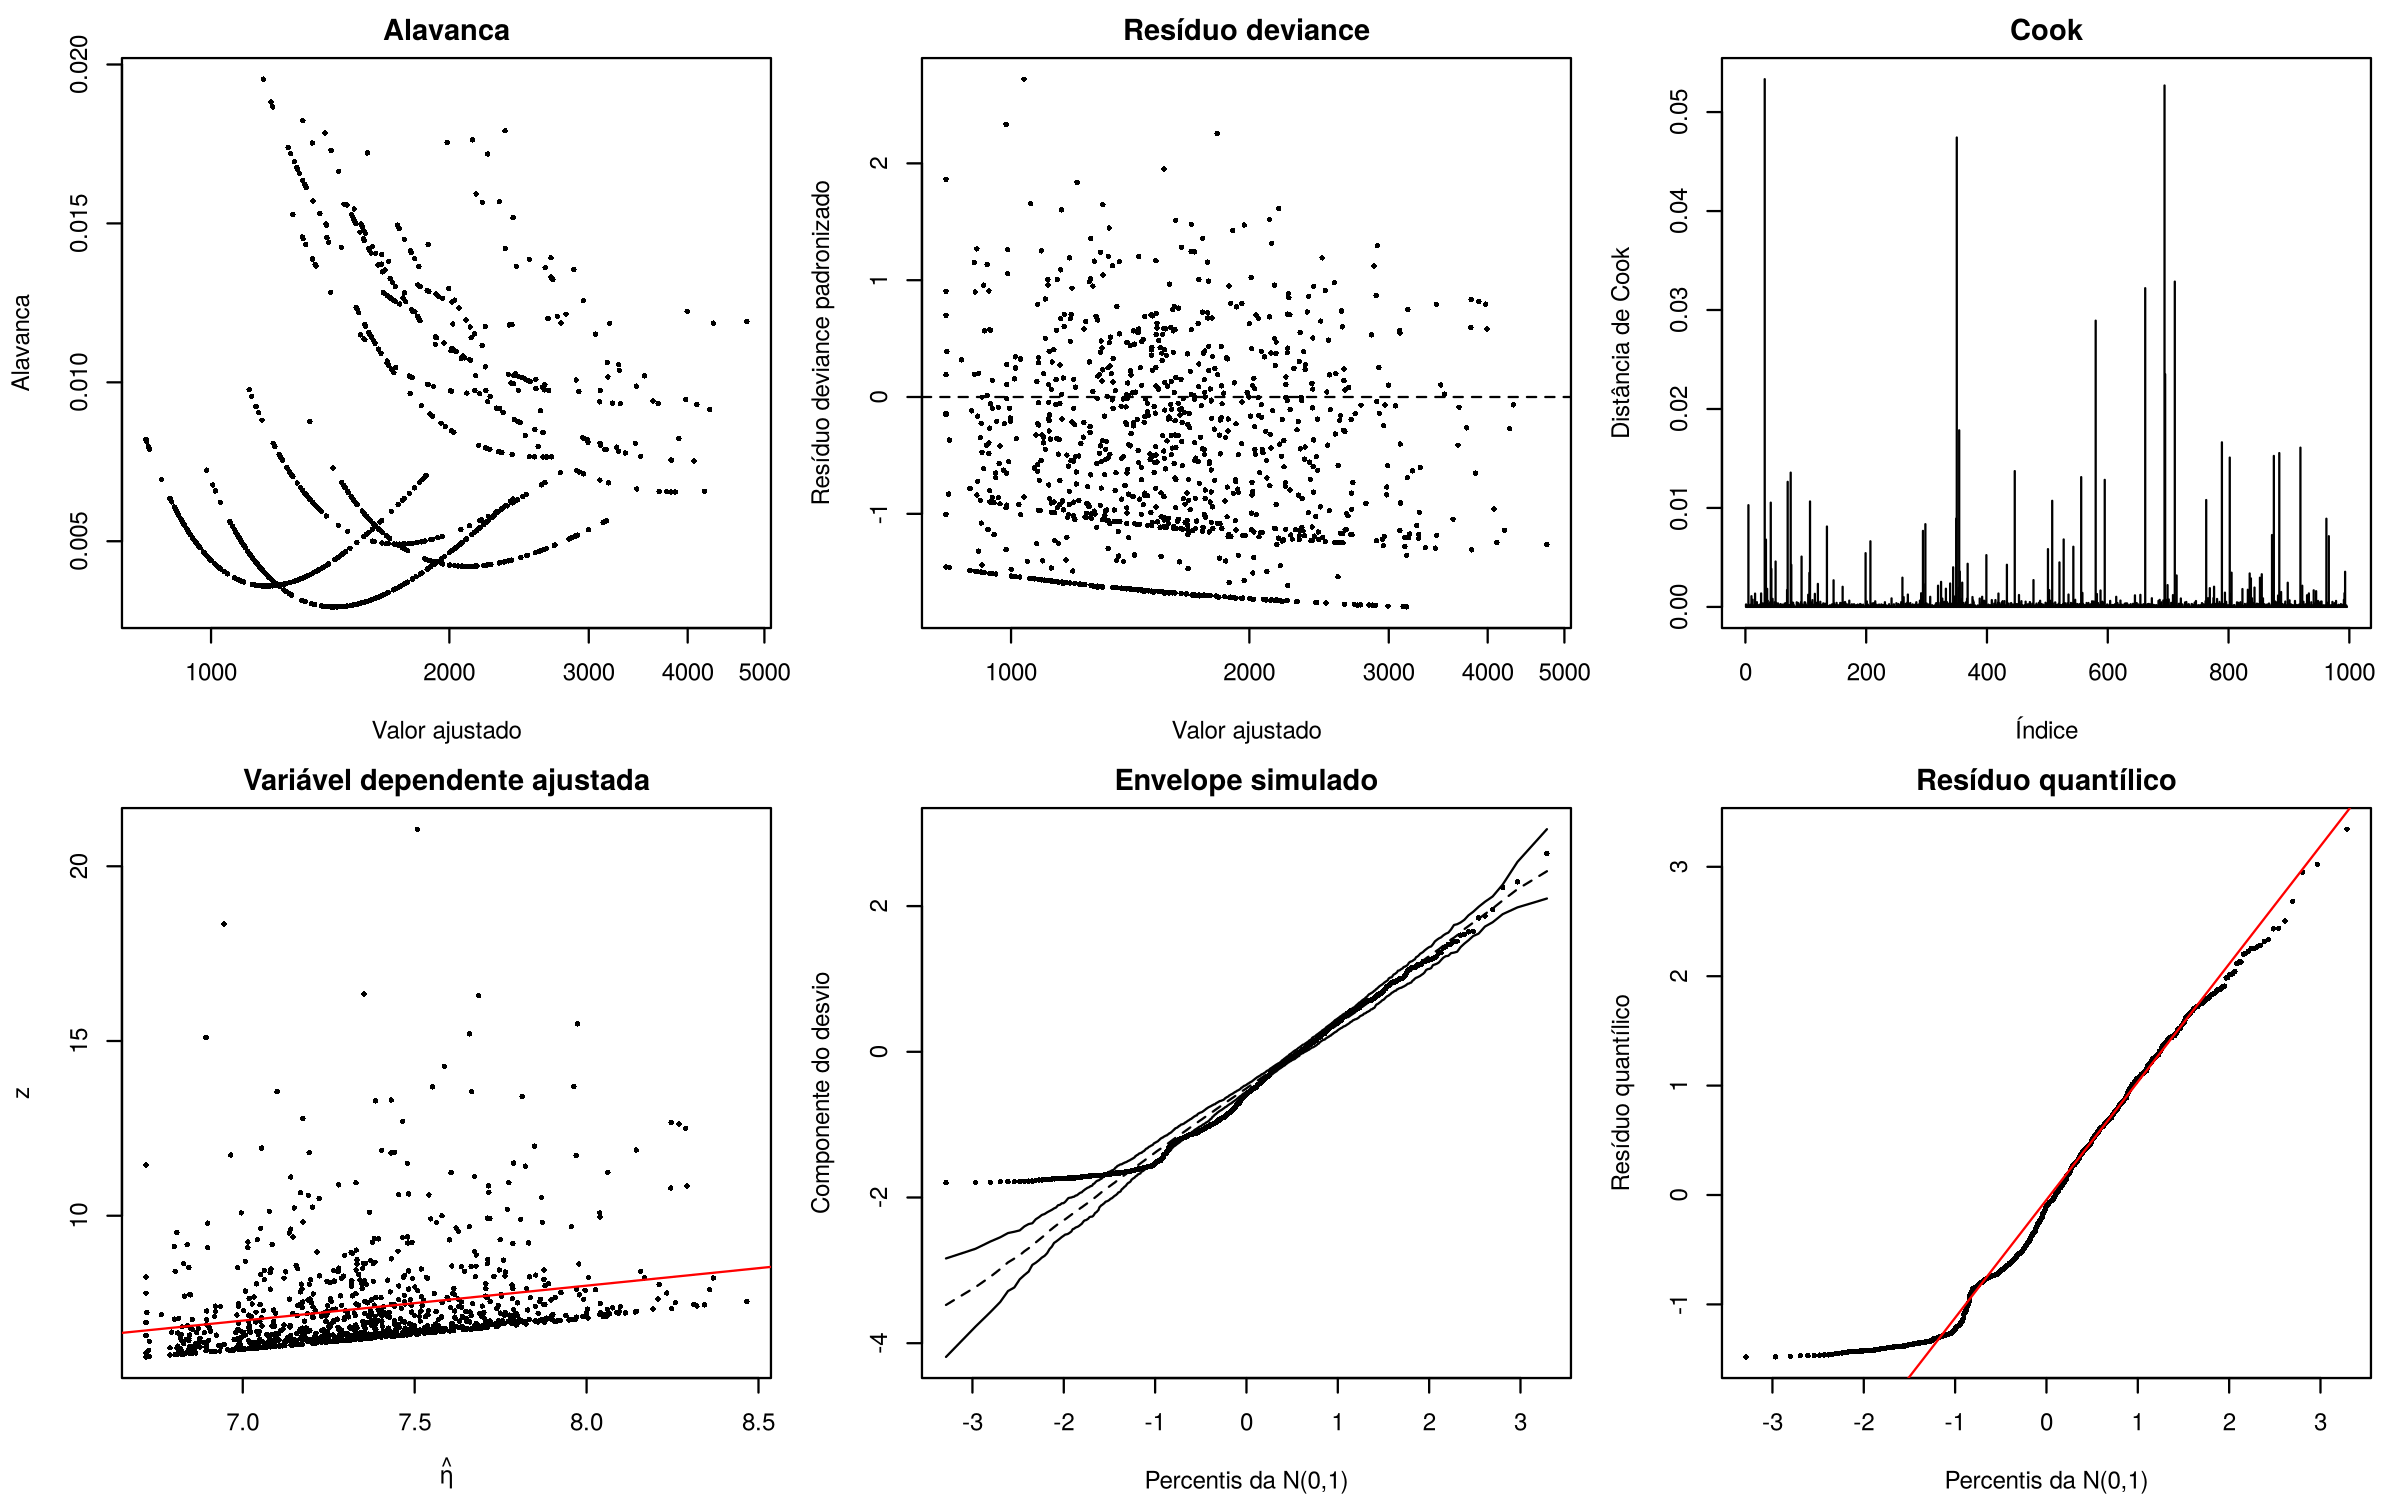
\includegraphics[width=0.92\textwidth]{ex1_diag_ni.png}
\caption{Diagnóstico do modelo normal inversa (ligação log): alavanca, resíduo deviance padronizado, distância de Cook, variável dependente ajustada contra $\hat\eta$, envelope simulado e gráfico normal do resíduo quantílico.}\label{fig:ex1diagni}
\end{figure}

O AIC da normal inversa é 437 unidades menor que o da gama (Tabela~\ref{tab:ex1comp}). No diagnóstico (Figura~\ref{fig:ex1diagni}), o resíduo quantílico fica próximo da N(0,1): média $-0{,}03$, desvio padrão 0,99 e assimetria 0,42, e o gráfico normal acompanha a reta em quase toda a faixa. No envelope, a parte central e a cauda superior ficam dentro das bandas. Os pontos que saem do envelope estão concentrados num patamar horizontal na cauda inferior, formado pelas apólices com custo 200. Trata-se de uma característica dos dados (valor mínimo repetido), que nenhuma distribuição contínua reproduz, e não de um problema no preditor. Não há padrão sistemático nos resíduos contra os valores ajustados, e a variável dependente ajustada $z=\hat\eta+\text{resíduo de trabalho}$ cresce com $\hat\eta$ de forma aproximadamente linear, sem indicar inadequação da ligação logarítmica. A variável \texttt{idadev2} fica no limite da significância ($p=0{,}057$), mas foi mantida para que os dois modelos tenham o mesmo preditor. Sua retirada não altera as demais conclusões. Conclui-se que o modelo normal inversa com ligação logarítmica é o mais adequado e ele foi adotado como modelo final.

\subsection*{Pontos alavanca, discrepantes e influentes}

\begin{figure}[H]
\centering
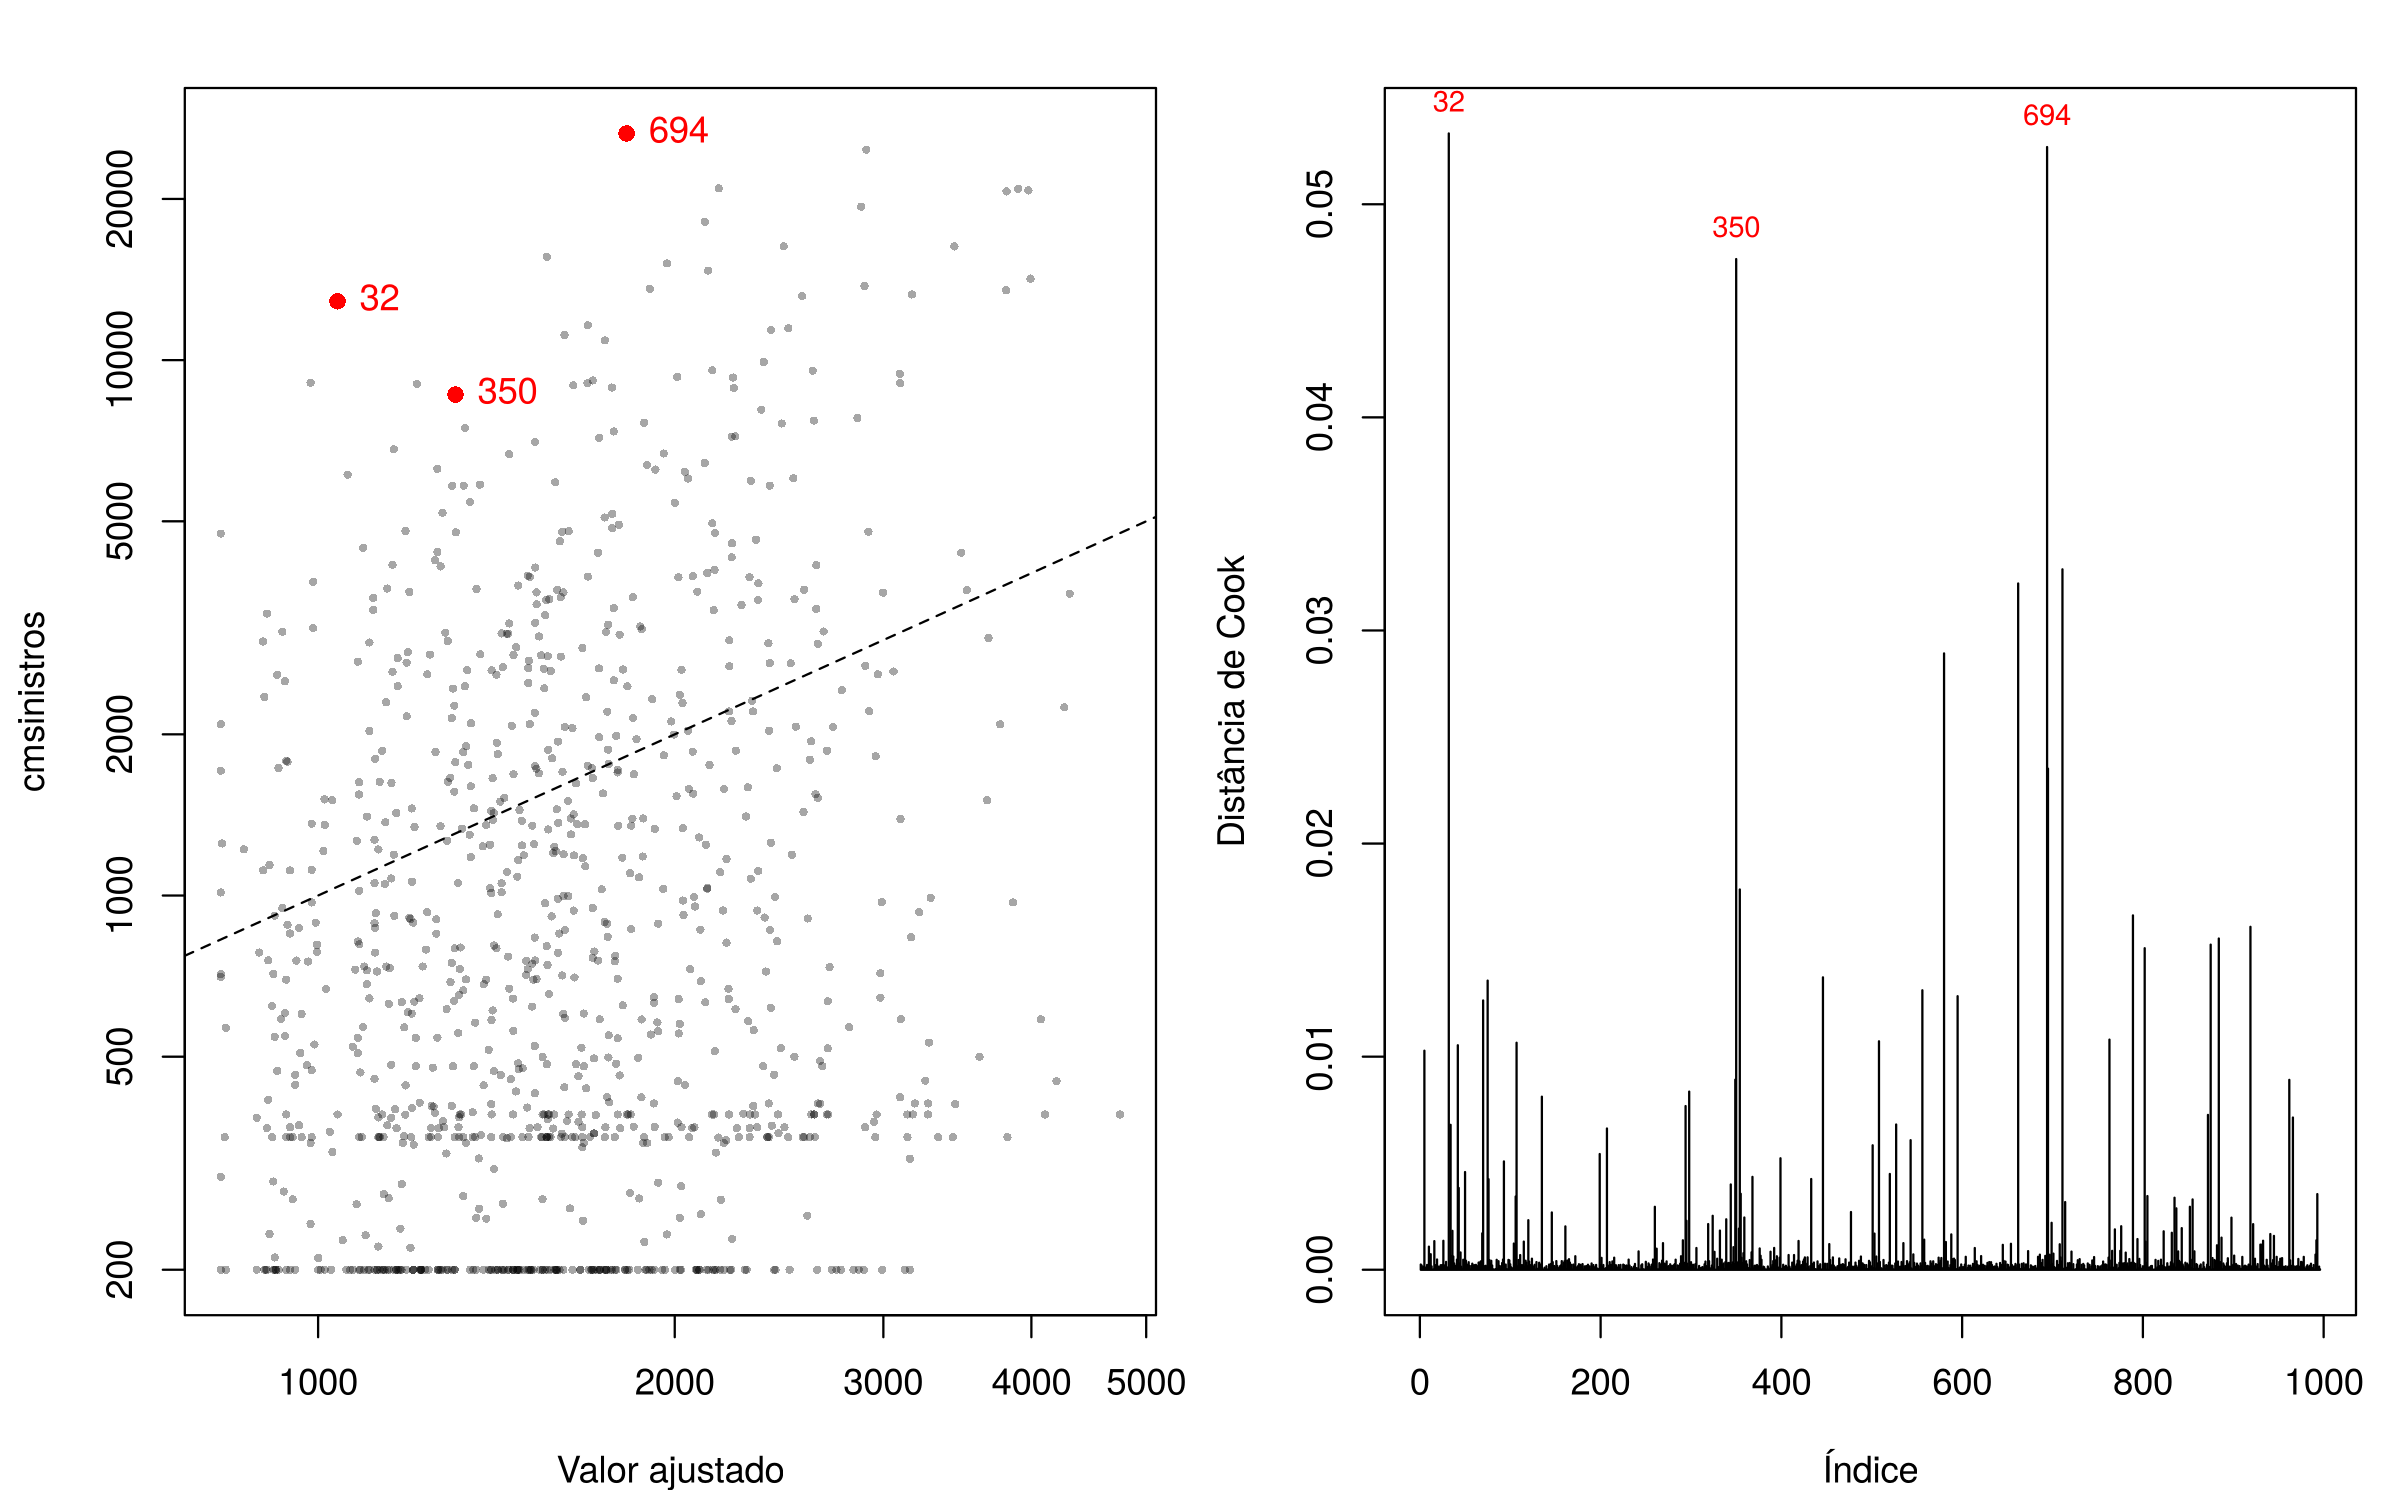
\includegraphics[width=\textwidth]{ex1_pontos.png}
\caption{Valor observado contra valor ajustado, em escala logarítmica (esquerda), e distância de Cook (direita) no modelo normal inversa. As observações destacadas estão em vermelho, numeradas pela linha.}\label{fig:ex1pontos}
\end{figure}

\begin{table}[H]
\centering\small
\caption{Observações destacadas no modelo normal inversa.}\label{tab:ex1pts}
\begin{tabular}{rrrlrrr}
\toprule
Obs. & \texttt{cmsinistros} & Ajustado & Perfil (tipo, idadev, área, idadec) & Alavanca & Res. deviance pad. & Cook \\
\midrule
32 & 12879,7 & 1038,5 & HBACK, 1, B, 3 & 0,004 & 2,72 & 0,053 \\
694 & 26507,3 & 1821,4 & STNWG, 2, C, 2 & 0,005 & 2,26 & 0,053 \\
350 & 8624,6 & 1306,1 & UTE, 1, A, 4 & 0,018 & 1,65 & 0,047 \\
\bottomrule
\end{tabular}
\end{table}

Como quase todas as preditoras são qualitativas, as alavancas formam faixas (uma para cada combinação de categorias) e são todas pequenas (máximo 0,020). Nenhum ponto se destaca como ponto de alta alavanca. Pelos gráficos de resíduos e de distância de Cook (Figuras~\ref{fig:ex1diagni} e \ref{fig:ex1pontos}), as observações 32, 694 e 350 se afastam das demais (Tabela~\ref{tab:ex1pts}):
\begin{itemize}[noitemsep]
\item \textbf{Linhas 32 e 694:} custos muito acima do esperado (cerca de 12 e 15 vezes o valor ajustado), com os maiores resíduos do banco e alavanca baixa, isto é, pontos discrepantes. São também os dois pontos de maior distância de Cook.
\item \textbf{Linha 350:} custo cerca de 6,6 vezes o esperado, com alavanca um pouco acima da típica (veículo UTE, pouco frequente) e a terceira maior distância de Cook, ou seja, moderadamente influente.
\end{itemize}

Para avaliar o efeito dessas observações, o modelo foi reajustado sem elas.

\begin{table}[H]
\centering\small
\caption{Estimativas do modelo normal inversa com todas as observações e sem as observações destacadas.}\label{tab:ex1sem}
\begin{tabular}{lrrrrr}
\toprule
Termo & Completo & Sem os pontos & Variação (\%) & $p$ completo & $p$ sem pontos \\
\midrule
Intercepto & 7,62881 & 7,55105 & $-1{,}0$ & $<0{,}001$ & $<0{,}001$ \\
\texttt{expos} & $-0{,}91086$ & $-0{,}90585$ & 0,6 & $<0{,}001$ & $<0{,}001$ \\
\texttt{tipov2} = outros & 0,34399 & 0,28160 & $-18{,}1$ & 0,043 & 0,072 \\
\texttt{idadev2} = 3--4 & 0,17666 & 0,25129 & 42,2 & 0,054 & 0,004 \\
\texttt{areac2} = E--F & 0,34971 & 0,38061 & 8,8 & 0,020 & 0,008 \\
\texttt{idadec2} = 1--2 & 0,30002 & 0,29749 & $-0{,}8$ & 0,005 & 0,003 \\
\texttt{idadec2} = 6 & 0,34124 & 0,38179 & 11,9 & 0,051 & 0,021 \\
\bottomrule
\end{tabular}
\end{table}

Ao retirar essas observações, as estimativas de \texttt{expos} e de \texttt{idadec2} = 1--2 praticamente não mudam (Tabela~\ref{tab:ex1sem}). A de \texttt{tipov2} diminui 18,1\% e deixa de ser significativa ao nível de 5\% ($p=0{,}072$), enquanto a de \texttt{idadev2} aumenta 42,2\% e passa a ser claramente significativa ($p=0{,}004$). Nenhum coeficiente muda de sinal, então as conclusões qualitativas se mantêm. Ainda assim, o efeito do tipo de veículo depende em parte dessas três apólices. Como os valores são legítimos (sinistros de custo alto ocorrem de fato), os pontos foram mantidos no modelo.

\subsection*{Pseudo $R^2$}

O pseudo $R^2$ baseado na deviance, $1-D(\hat\mu)/D_0$, é 0,056 para o modelo normal inversa (0,095 para o gama), e o quadrado da correlação entre $\hat\eta$ e $\log(\texttt{cmsinistros})$ é 0,033. O poder explicativo é baixo: as covariáveis disponíveis explicam pouco da variação do custo de um sinistro individual, que é muito variável. Isso não invalida o modelo, cujo objetivo é estimar como o custo \emph{médio} varia entre os perfis, mas mostra que a previsão para uma apólice específica é imprecisa. Os dois pseudo $R^2$ não devem ser usados para comparar os modelos, pois as deviances da gama e da normal inversa estão em escalas diferentes.

\subsection*{Interpretação do modelo final}

\begin{table}[H]
\centering\small
\caption{Estimativas do modelo final (normal inversa, ligação logarítmica). Os testes e intervalos usam a distribuição $t$ com 989 graus de liberdade.}\label{tab:ex1coef}
\begin{tabular}{lrrrrrl}
\toprule
Termo & Estimativa & EP & $t$ & $p$ & $\exp(\hat\beta)$ & IC 95\% para $\exp(\beta)$ \\
\midrule
Intercepto & 7,62881 & 0,15171 & 50,28 & $<0{,}001$ & 2056,606 & (1527,055; 2769,796) \\
\texttt{expos} & $-0{,}91086$ & 0,19293 & $-4{,}72$ & $<0{,}001$ & 0,40218 & (0,27542; 0,58728) \\
\texttt{tipov2} = outros & 0,34399 & 0,16979 & 2,03 & 0,043 & 1,41056 & (1,01085; 1,96833) \\
\texttt{idadev2} = 3--4 & 0,17666 & 0,09175 & 1,93 & 0,054 & 1,19323 & (0,99663; 1,42861) \\
\texttt{areac2} = E--F & 0,34971 & 0,15052 & 2,32 & 0,020 & 1,41866 & (1,05585; 1,90614) \\
\texttt{idadec2} = 1--2 & 0,30002 & 0,10702 & 2,80 & 0,005 & 1,34989 & (1,09419; 1,66533) \\
\texttt{idadec2} = 6 & 0,34124 & 0,17443 & 1,96 & 0,051 & 1,40670 & (0,99896; 1,98086) \\
\bottomrule
\end{tabular}
\end{table}

A dispersão estimada é $\hat\phi=$ 0,00137. Com ligação logarítmica, $\exp(\hat\beta_j)$ é o fator multiplicativo no custo médio por sinistro associado ao aumento de uma unidade da preditora $j$ (ou à mudança da categoria de referência para a categoria indicada), com as demais fixas. Assim:
\begin{itemize}[noitemsep]
\item Cada aumento de 0,1 na exposição multiplica o custo médio por $\exp(-0{,}0911)=0{,}913$ (redução de 8,7\%), mantidas as demais variáveis fixas. Apólices com exposição curta que tiveram sinistro tendem a ter sinistros mais caros;
\item Veículos de tipo menos comum (utilitários, vans, caminhões, cupês, ônibus) têm custo médio 41,1\% maior que os de tipo comum, mantidas as demais variáveis fixas;
\item Veículos com idade nas classes 3--4 têm custo médio 19,3\% maior que os das classes 1--2, mantidas as demais variáveis fixas (efeito no limite da significância);
\item Condutores residentes nas áreas E e F têm custo médio 41,9\% maior que os das áreas A a D, mantidas as demais variáveis fixas;
\item Condutores jovens (classes 1--2) têm custo médio 35,0\% maior, e os mais velhos (classe 6) custo médio 40,7\% maior (no limite da significância), que os de idade intermediária (classes 3--5), mantidas as demais variáveis fixas.
\end{itemize}

Para uma exposição igual à mediana (0,616) e veículo com idade nas classes 1--2, o custo médio previsto vai de 1173 dólares australianos (veículo comum, áreas A--D, condutor de idade intermediária) a 3303 dólares australianos (veículo de outro tipo, áreas E--F, condutor da classe 6), uma diferença de cerca de 2,8 vezes.
